%==================================================================%
% Author : Pando Muñoz, Manuel                                     %
%          Sánchez Barreiro, Pablo                                 %
% Version: 1.0, 02/03/2011                                         %
%                                                                  %
% Memoria del Proyecto Fin de Carrera                              %
% Archivo raíz para el capítulo de iteración                       %
%==================================================================%

\chapterheader{Segunda iteración}{Descripción de una iteración}
\label{chap:iteracion}

\chaptertoc

En el siguiente capítulo se describe lo realizado en la segunda iteración de construcción.
Se parte de lo obtenido en las iteraciones previas, que es, la descripción del sistema, la arquitectura del mismo y los diagramas de secuencia y estados, todo esto expuesto a lo largo de los capítulos \ref{chap:planificacion} y \ref{chap:arquitectura}.
\newline

En cuanto al estado de la aplicación, en la primera iteración de construcción se ha desarrollado un sistema distribuido, en el que desde la aplicación del alumno se puede conectar con la aplicación del profesor y transmitir ficheros.
\newline

El objetivo de esta iteración es que el profesor pueda establecer el inicio y de la prueba, poder prefijar una hora de finalización de la misma y que la aplicación del alumno sea capaz de denegar el acceso a la red mientras dure la prueba.
\newline

En la tabla \ref{tabla:objetivosIteracion} se pueden ver los requisitos a implementar durante esta iteración y en la \ref{tabla:baseIteracion} la base, o lo que es lo mismo, lo implementado en la iteración anterior. La lista global de requisitos se encuentra en la tabla \ref{tabla:requisitos}.
\newline

En las siguientes secciones se describen los incrementos realizados dentro de esta iteración, generalmente coincide el número de incrementos en cada iteración con el número de requisitos a implementar.

\begin{table}
\begin{tabular}{|c|p{10cm}|}
	\hline
	\textbf{Identificador} & \textbf{Descripción}
	\\ \hline
	
	R03 & El profesor debe ser capaz desde el \emph{Watchman} de indicar el inicio de la prueba.
	\\ \hline

	R05 & El profesor ha de ser capaz desde el \emph{Watchman} de establecer una hora límite para la duración de la prueba.
	\\ \hline

	R10 & El alumno desde su computador debe tener la posibilidad de ver el tiempo restante el pruebas de duración prefijada.
	\\ \hline

	R11 & La aplicación del alumno ha de ser capaz de denegar el acceso a la red al empezar la prueba.
	\\ \hline
	
\end{tabular}
\label{tabla:objetivosIteracion}
\caption{Objetivos de la iteración}
\end{table}

\begin{table}
\begin{tabular}{|c|p{10cm}|}
	\hline
	\textbf{Identificador} & \textbf{Descripción}
	\\ \hline

	R01 & Un computador de la red debe poder ser designado como \emph{Watchman}.
	\\ \hline

	R02 & Todos los computadores que no sean \emph{Watchman} serán computadores
	normales, y podrán ser utilizados para la realización de las pruebas evaluables.
	\\ \hline

	R06 & El profesor debe ser capaz desde el \emph{Watchman} de enviar el fichero de enunciado al resto de computadores.
	\\ \hline

	R07 & El alumno desde su computador debe ser capaz de conectarse al \emph{Watchman}.
	\\ \hline

	R13 & La aplicación ha de ser capaz de comprobar que los archivos se han enviado correctamente.
	\\ \hline

\end{tabular}
\label{tabla:baseIteracion}
\caption{Requisitos ya implementados del sistema}
\end{table}


\section{Inicio de la prueba}
\label{sec:iteracion:iniPrueba}

En esta sección se comenta cómo se consigue que el profesor pueda notificar a los alumnos el inicio de la prueba.
Como ya hemos comentado, partimos de la iteración anterior en la cual los alumnos eran capaces de conectar a la aplicación del profesor. En la aplicación del alumno, cuando se crea una conexión, se inicia a su vez un hilo de ejecución que se mantiene a la espera de recibir distintas órdenes provenientes del computador del profesor. De este modo se hace muy simple mantener desde la aplicación del profesor una lista de las conexiones abiertas con cada alumno y, al presionar el botón de iniciar la prueba, recorrer esa lista enviando la orden por cada conexión.
Cuando cada una de las aplicaciones del alumno recibe esa orden, actúa en consecuencia.

\section{Examen temporizado}
\label{sec:iteracion:examenTemporizado}

El profesor puede establecer una hora límite, llegada la cual, la prueba terminará automáticamente. Cuando el profesor define este límite en su aplicación y decide comenzar la prueba se envía también si hay una hora de fin y, en caso afirmativo, cual es. De este modo la aplicación del alumno puede mostrar una cuanta atrás con los minutos restantes para la finalización, para facilitar la referencia temporal. Se puede ver el resultado en la siguiente imagen.

\begin{figure}[!htb]
    \centering
    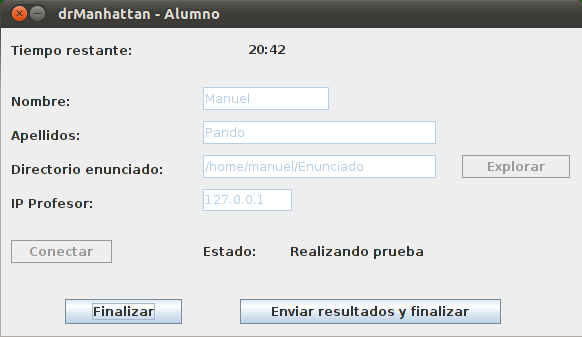
\includegraphics[width=.90\linewidth]{iteracion/tiempoRestante}
    \caption{Aspecto de la GUI del alumno con una prueba temporizada.}
    \label{fig:iteracion:tiempoRestante}
\end{figure}


\section{Denegar acceso a red}
\label{sec:iteracion:denegarRed}

Cómo ya hemos visto en las secciones anteriores, una vez que la aplicación del alumno recibe la orden de comenzar la prueba, se ha de denegar el acceso a la red. Para ello se utiliza iptables, por medio de un demonio.
\newline

El demonio creado es muy simple, se ejecuta en segundo plano esperando a que la aplicación del alumno conecte, y en función de lo requerido en ese momento, permitir o no el acceso a la red interactuando con iptables. Este demonio se inicia en tiempo de arranque y con los permisos necesarios para poder usar el cortafuegos.
\newline

Las órdenes concretas que ejecuta el demonio son, cuándo se desea denegar la red son:

\begin{center}

    \emph{iptables -P OUTPUT DROP}

    \emph{iptables -A OUTPUT -s 127.0.0.1 -j ACCEPT}

\end{center}

Con la primera de ellas se cambia la política del tratamiento a los paquetes salientes del equipo, de modo que los deseche, dicho de otro modo, no se permiten las comunicaciones salientes con otros computadores, de esta forma se evita que se hagan peticiones, por ejemplo, a un servidor web.
\newline

La segunda es para permitir los paquetes salientes dirigidos al propio ordenador. Esto es necesario para la comunicación entre la aplicación del alumno y el demonio.
\newline

Puede parecer que el equipo queda totalmente aislado, incluso del computador del profesor, pero esto no es así, puesto que ya hay una conexión establecida y dado que la aplicación del alumno espera órdenes de la aplicación del profesor, puede seguir funcionando perfectamente, puesto que los paquetes de entrada sí que están permitidos, lo que estas instrucciones imposibilitan es la creación de nuevas conexiones y el envío de mensajes a cualquier computador que no sea el propio.


\section{Pruebas}
\label{sec:iteracion:pruebas}

En esta sección se describen las pruebas realizadas en la iteración con el objetivo de determinar si el funcionamiento de lo construido es correcto.
\newline

Debido a la naturaleza del sistema, automatizar pruebas con una herramienta estilo \emph{JUnit} es prácticamente imposible, ya que funciona a base de eventos y es distribuido, por eso, para probar la aplicación utilizo el equipo de sobremesa y un portátil, para intentar recrear el entorno del laboratorio y ejecuto secuencias de acciones para desencadenar los eventos requeridos en cada funcionalidad.

\begin{itemize}

	\item {\bfseries R03} - El profesor debe ser capaz desde el \emph{Watchman} de indicar el inicio de la prueba.

    \begin{itemize}

        \item Pulsar el botón y ver que efectivamente llega la señal al computador del alumno.

    \end{itemize}

    \item {\bfseries R05} - El profesor ha de ser capaz desde el \emph{Watchman} de establecer una hora límite para la duración de la prueba.

    \item {\bfseries R10} - El alumno desde su computador debe tener la posibilidad de ver el tiempo restante el pruebas de duración prefijada.

    \begin{itemize}
        \item Establecer horas correctas futuras y comprobar que los minutos calculados restantes son correctos.

        \item Establecer horas pasadas y comprobar que no se temporiza la prueba.

        \item Establecer horas incorrectas y comprobar que es detectado.
    \end{itemize}


    \item {\bfseries R11} - La aplicación del alumno ha de ser capaz de denegar el acceso a la red al empezar la prueba.

    \begin{itemize}

        \item Después de que de inicio la prueba, en el computador del alumno, intentar abrir páginas web en el navegador, pings a equipos.
    \end{itemize}

\end{itemize} 